\documentclass[journal,12pt,twocolumn]{IEEEtran}
\usepackage{graphicx}
\graphicspath{{./figs/}}{}
\usepackage{amsmath,amssymb,amsfonts,amsthm}
\newcommand{\myvec}[1]{\ensuremath{\begin{pmatrix}#1\end{pmatrix}}}
\usepackage{listings}
\usepackage{watermark}
\usepackage{titlesec}
\let\vec\mathbf
\lstset{
frame=single, 
breaklines=true,
columns=fullflexible
}
\thiswatermark{\centering \put(0,-105.0){
\includegraphics[scale=0.5]{iith.png}} }

\title{\mytitle}
\title{
Matrix Assignment - Lines
}
\author{Nikhil Nair}
\begin{document}
\maketitle
\tableofcontents
\bigskip


\section{\textbf{Problem}}
Find the orthocenter of triangle with vertices (0,0), (3,4) and (4,0).\\


\section{\textbf{Solution}}
Orthocenter of a triangle is the point where perpendiculars drawn to the opposite side from each vertex of the triangle intersect.   \\
\\
To find the orthocenter first we find the coordinates of point Q i.e the foot of the perpendicular drawn from point B as follows\\
\\

${\vec{OA}}=O + \lambda.\vec{
  m}$
\\

where O is the origin and $\vec{m}= A-O$
\\
\begin{equation}
 \vec{OA}=\lambda.\myvec{
  3\\
  4}     \label{eq-1}
\end{equation}
\\
Now, 
\\

${\vec{m^{\top}}(\vec{OA}-B)} = 0$
\\
\\	

 $\vec{m^{\top}}[O + \lambda.\vec{m} - B ]= 0 $ 
\\
\\

$\lambda.{\lVert m \rVert}^2 = \vec{m^{\top}}(O-B)$
\\
\\
\begin{equation}
	\lambda=\frac{\vec {m^{\top}}(O-B)}{{\lVert m \rVert}^2} 
	\label{eq-2}
\end{equation}
\\
Coordinates of Point Q can be found by replacing value of $\lambda$ in eq 2
\\
\\

$ Q = \frac{\vec{m^{\top}}(O-B)}{{\lVert m \rVert}^2}  . \myvec{
  3\\
  4} $ 
\\
\\

$ Q=\frac{1}{\surd(3^2 + 4^2)}\myvec{
  3\
  4}\myvec{
  4\\
  0}\myvec{
  3\\
  4} $ 
\\  
\\

$ Q=\myvec{
  1.44\\
  1.92} $ 
\\  
 \\
 
 The orthocenter of the triangle can be calculated as follows
 \\
 
 From the points,\\
 
 A( 3, 4 )     ;        P( 3, 0 )
 
 B( 4, 0 )     ;        Q( 1.44, 1.92 )
 
 
 
 \begin{equation}
 \vec{AP} = \myvec{3\\4}+\lambda1. \myvec{ 0\\-4}
 \end{equation}




\begin{equation}
\vec{BQ} = \myvec{4\\0}+\lambda2. \myvec{-2.56\\1.92}
\end{equation}
  \\
  
  where $\lambda1$ and $\lambda2$ are scalars
  \\  
 \vspace{4cm}
 \\
 Solving eq3 and eq4 we get the value of 
 \\
 \begin{center}
 $\lambda2$ = 0.39
 \end{center}
 \vspace{0.5cm}
 
  Replace the value of $\lambda2$ in eq4 to find the intersection of 
  $\vec{AP}$ and $\vec{BQ}$ , ie point X.
\vspace{1cm}
\\

X = $\myvec{4\\0}+ 0.39. \myvec{-2.56\\1.92}$
\\
\\
\vspace{0.3cm}

Therefore the orthocenter of the triangle is
\\

X = $\myvec{3\\0.75}$
\\

\section{\textbf{Figure}}
\begin{figure}[h]
    \centering
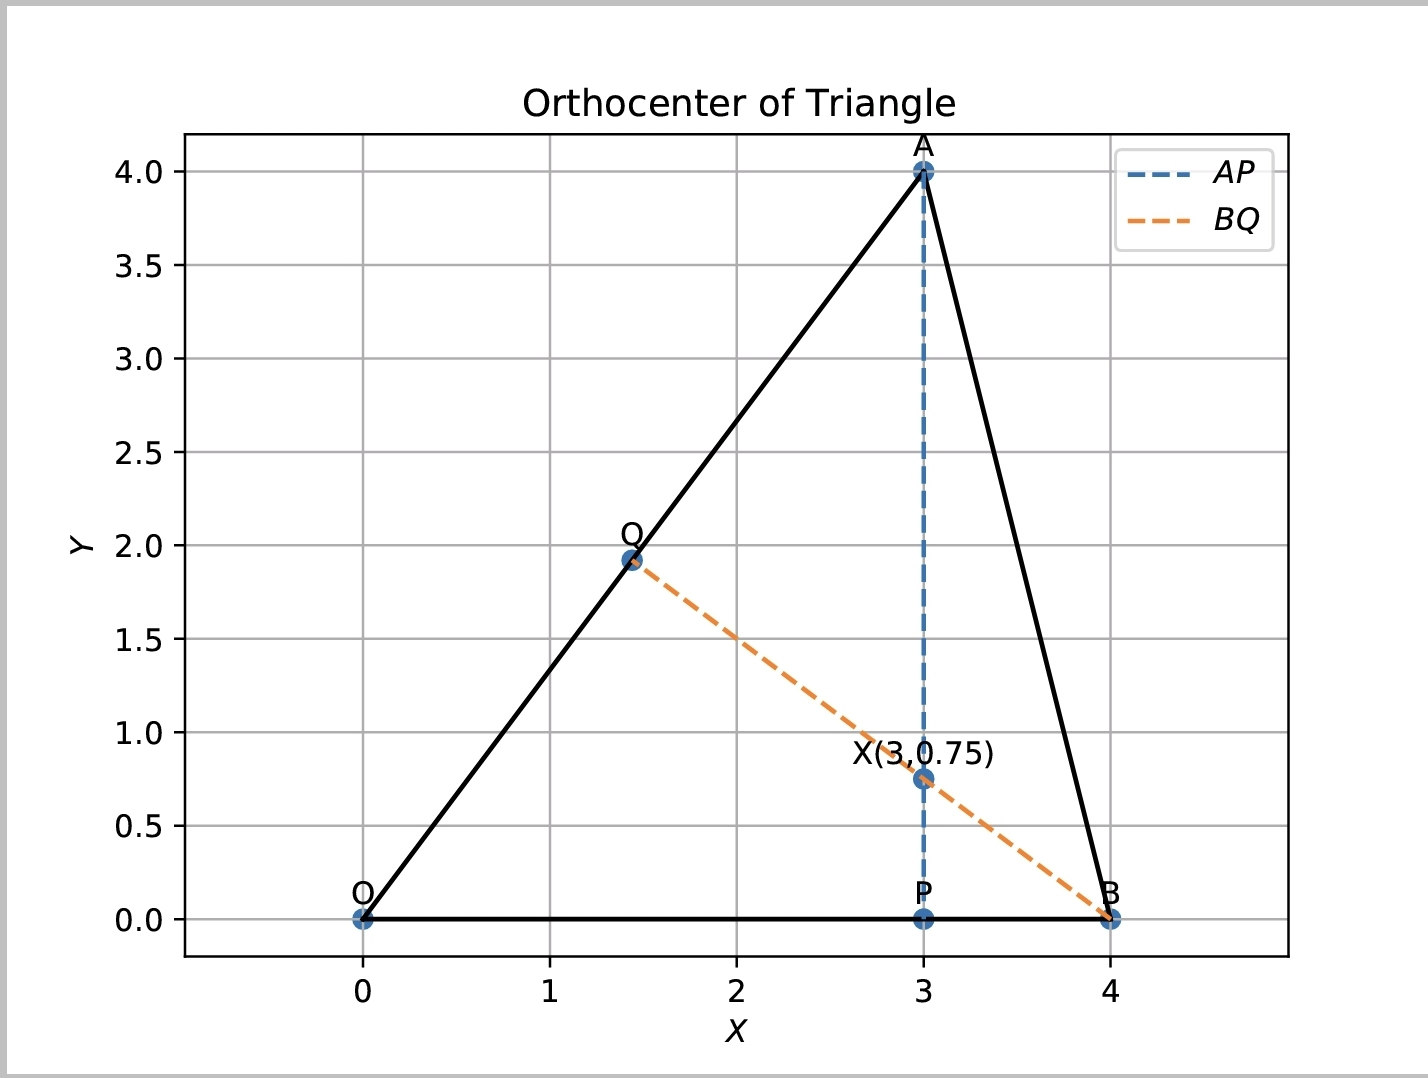
\includegraphics[width=\columnwidth]{fig.jpg}
    \label{fig:my_label}
\end{figure}


\section{\textbf{Code Link}}

\begin{lstlisting}
https://github.com/nikhilnair90/FWC-2/blob/main/Matrix/Line/line.py
\end{lstlisting}
Execute the code by using the command\\
\textbf{python3 line.py}



\end{document}
